%% gtile_part.tex
\newpage
\subsection{Glass Tile}

\paragraph{Beschreibung des Filters aus Nutzersicht}

Dieses Filter lässt das Bild erscheinen, als würde es durch eine Wand aus Glasbausteinen betrachtet werden. Das Filter kann auf die aktive Ebene oder eine im Bild befindliche Auswahl angewendet werden.\footnote{\url{http://docs.gimp.org/de/plug-in-glasstile.html}} Die Kachelbreite und Kachelhöhe sind individuell einstellbar.

\paragraph{Algorithmus}

%Pseudocode, visuell
\begin{algorithm}[h]
\caption{Pseudo-Code des \glqq Glass Tile\grqq-Algorithmus}
\label{algo:gtile}
\begin{algorithmic}[1]
\State $xhalf \gets tileWidth  / 2$
\State $yhalf \gets tileHeight / 2$
\State $xplus \gets tileWidth  \mod 2$
\State $yplus \gets tileHeight \mod 2$
\State $ymiddle \gets 0$
\State $yoffs \gets 0$
\ForAll{$rows$ $r$ $\in input$}
	\State $ypixel2 \gets ymiddle + yoffs * 2$
	\State lese Zeile $ypixel2$ aus dem Eingabebild
	\State $yoffs$++
	\If{$yoffs = yhalf$}
		\State{$ymiddle \gets ymiddle + tileHeight$}
		\State{$yoffs \gets - (yhalf + yplus)$}
	\EndIf
	\State $xmiddle \gets 0$
	\State $xoffs \gets 0$
	\ForAll{$columns \in column$}
		\State $xpixel1 \gets (xmiddle + xoffs)$
		\State $xpixel2 \gets (xmiddle + xoffs * 2)$
		\State schreibe Pixel $xpixel2$ aus Eingabezeile nach $xpixel1$ in Ausgabezeile
		\State $xoffs$++
		\If{$xoffs = xhalf$}
			\State{$xmiddle \gets xmiddle + tileWidth$}
			\State{$xoffs \gets - (xhalf + xplus)$}
		\EndIf
	\EndFor
	\State speichere Ausgabezeile an Zeilenposition $r$ im Ausgabebild
\EndFor	
\end{algorithmic}
\end{algorithm}

%Beschreibung Algorithmus allgemeinsprachlich
\begin{figure}[h]
\begin{center}
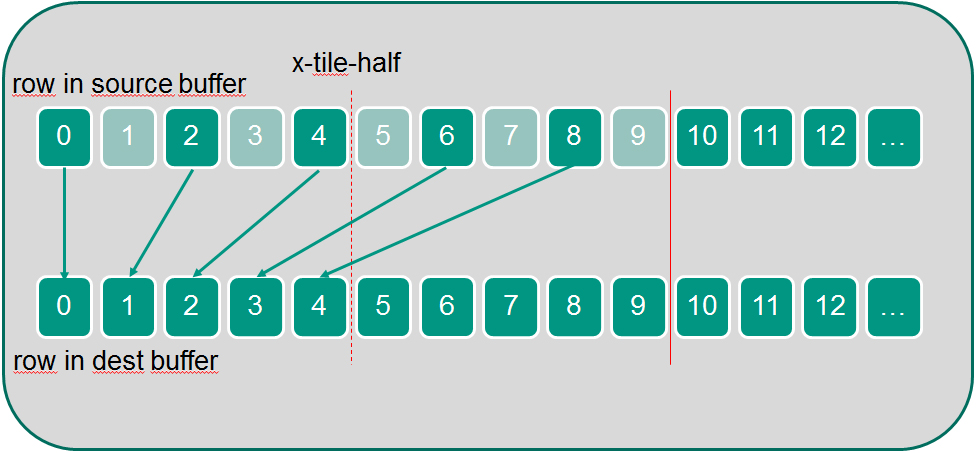
\includegraphics[width=0.95\textwidth]{gtile1.png}
\end{center}
\caption{Verrückung der Spalten innerhalb einer Zeile}\label{fig:gtile1}
\end{figure}
Der Algorithmus erzeugt sowohl zeilenweise als auch spaltenweise eine Verrückung und Wiederholung innerhalb der Kacheln. Dabei wird jede zweite Zeile in einer Kachel hintereinander in die erste Hälfte der Kachel verschoben wie in Abbildung~\ref{fig:gtile1} zu sehen.\newline
\begin{figure}[h]
\begin{center}
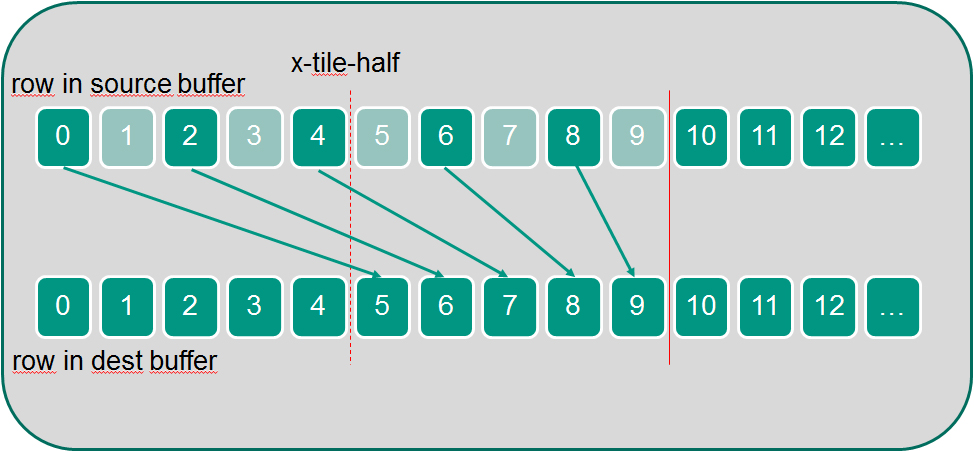
\includegraphics[width=0.95\textwidth]{gtile2.png}
\end{center}
\caption{Wiederholung der verrückten Spalten innerhalb einer Kachelzeile}\label{fig:gtile2}
\end{figure}
Diese gelesenen und verschobenen Zeilen werden anschließend in der zweiten Hälfte nochmals wiederholt, was in Abbildung~\ref{fig:gtile2} dargestellt ist.\newline
Die Verrückung und Wiederholung der Spalten erfolgt analog. Auf diese Weise wird Kachel für Kachel bearbeitet. Der sequentielle original Algorithmus liest dabei komplette Zeilen ein und führt darauf die notwendigen Spaltenverschiebungen durch.

\paragraph{Portierung}
Bei der Portierung wurde etwas getan.

\paragraph{Parallelisierung}
Peinlich peinlich möchte man denken.